\section*{Overview}

Rotating calipers is the geometry pattern for convex polygons when one pointer is not enough but restarting the second
pointer from scratch would waste too much work. The picture is two supporting lines rotating together, but the contest
implementation is usually just a monotone pointer on hull indices.

\section*{When to Use It}

Use it when:

\begin{itemize}
  \item the input is already a convex polygon or can be reduced to one by taking the convex hull,
  \item the interesting pair or edge moves monotonically around the hull,
  \item you need diameter, width, farthest pair, or another antipodal-style quantity.
\end{itemize}

\section*{Core Idea}

For convex polygons, as one edge advances to the next edge in cyclic order, the best opposing point also advances in
cyclic order. That monotonicity turns an apparent \(O(n^2)\) pair scan into \(O(n)\) after the hull is known.

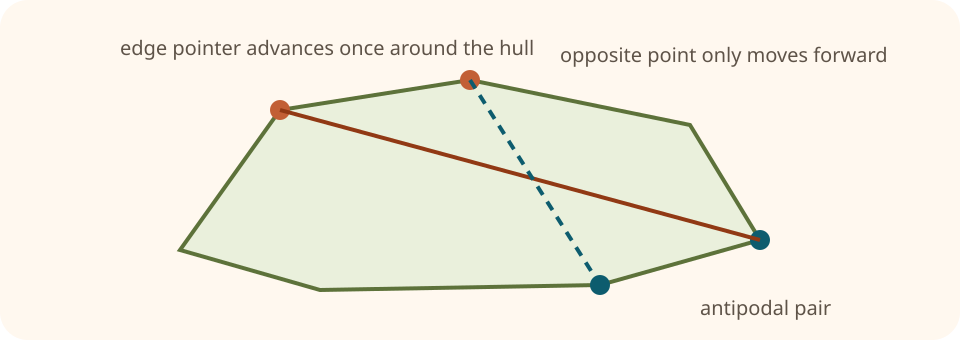
\includegraphics[width=\textwidth]{figures/antipodal-pairs.svg}

\section*{Key Insight}

The second pointer never needs to move backward. This is the exact geometric analog of a two-pointer proof on arrays:
the objective changes smoothly enough that once an index stops being optimal, it will not become optimal again later.

\section*{Worked Problem}

\paragraph{Problem.}
Given \(n\) points in the plane, find the maximum squared distance between any two points.

\paragraph{Why calipers fit.}
The farthest pair must be on the convex hull. After building the hull, the diameter can be found by scanning antipodal
pairs with one advancing pointer.

\paragraph{Algorithm outline.}

\begin{itemize}
  \item Build the convex hull in counterclockwise order.
  \item For each hull edge \((i, i+1)\), advance pointer \(j\) while the area with \(j+1\) increases.
  \item Check the relevant pair distances for \(i\) and \(j\).
\end{itemize}

\section*{Correctness Intuition}

Advancing \(j\) while the signed area increases keeps the opposite supporting line as far as possible from edge
\((i,i+1)\). Convexity guarantees that once the area starts decreasing, further advancing \(j\) cannot help for the same
edge, and the next edge only moves the optimum forward.

\section*{Complexity Analysis}

After the hull is built in \(O(n \log n)\), the calipers scan is \(O(h)\), where \(h\) is the hull size.

\section*{Implementation}

The code assumes the convex hull is already built and returns the squared diameter of that hull.

\section*{Common Pitfalls}

\begin{itemize}
  \item Running calipers on a non-convex polygon.
  \item Forgetting cyclic indexing on the hull.
  \item Mishandling small hull sizes \(h \le 2\).
  \item Comparing floating-point distances when integer squared distance is enough.
\end{itemize}

\section*{Variants / Extensions}

\begin{itemize}
  \item Minimum width of a convex polygon.
  \item Maximum area triangle on a convex polygon.
  \item Farthest pair between two convex polygons under specialized setups.
\end{itemize}

\section*{Practice Problems}

\begin{itemize}
  \item Diameter of a point set.
  \item Width or thickness of a convex polygon.
  \item Any hull problem where the optimal opposing point moves monotonically.
\end{itemize}

\section*{References}

\begin{itemize}
  \item \href{https://cp-algorithms.com/geometry/rotating_calipers.html}{cp-algorithms: Rotating Calipers}.
  \item \href{https://usaco.guide/plat/geo-ext}{USACO Guide: Extra Geometry}.
  \item \href{https://codeforces.com/catalog}{Codeforces Catalog}.
\end{itemize}
